% !TEX TS-program = pdflatex
% !TEX encoding = UTF-8 Unicode

\documentclass[12pt,oneside]{book} % use larger type; default would be 10pt

\usepackage[utf8]{inputenc} % set input encoding (not needed with XeLaTeX)

\usepackage[parfill]{parskip} % paragraph breaks with lines

\usepackage{csquotes}

\usepackage{lipsum}%

\usepackage[svgnames]{xcolor}

%%% Examples of Article customizations
% These packages are optional, depending whether you want the features they provide.
% See the LaTeX Companion or other references for full information.

%%% Copyright SECTION
\usepackage{fancyhdr}
\def\secondpage{\clearpage\null\vfill
\pagestyle{empty}
\begin{minipage}[b]{0.9\textwidth}
\footnotesize\raggedright
\setlength{\parskip}{0.5\baselineskip}
Copyright \copyright 2020--\the\year\ by Zachary Calvert\par
All rights reserved.
\end{minipage}
\vspace*{2\baselineskip}
\cleardoublepage
\rfoot{\thepage}}

\makeatletter
\g@addto@macro{\maketitle}{\secondpage}
\makeatother


%%% PAGE DIMENSIONS
\usepackage[papersize={8.5in,11in}]{geometry}
% \usepackage{geometry} % to change the page dimensions
% \geometry{a5paper} % or letterpaper (US) or a5paper or....
\geometry{margin=1in} % for example, change the margins to 2 inches all round
% \geometry{landscape} % set up the page for landscape
%   read geometry.pdf for detailed page layout information

\usepackage{graphicx} % support the \includegraphics command and options
\graphicspath{ {./uml/} }

%%% PACKAGES
\usepackage{booktabs} % for much better looking tables
\usepackage{array} % for better arrays (eg matrices) in maths
\usepackage{paralist} % very flexible & customisable lists (eg. enumerate/itemize, etc.)
\usepackage{verbatim} % adds environment for commenting out blocks of text & for better verbatim
\usepackage{subfig} % make it possible to include more than one captioned figure/table in a single float
% These packages are all incorporated in the memoir class to one degree or another...
\usepackage{hyperref}

%%% HEADERS & FOOTERS
\usepackage{fancyhdr} % This should be set AFTER setting up the page geometry
\pagestyle{fancy} % options: empty , plain , fancy
\renewcommand{\headrulewidth}{0pt} % customise the layout...
\lhead{}\chead{}\rhead{}
\lfoot{}\cfoot{\thepage}\rfoot{}

%%% SECTION TITLE APPEARANCE
\usepackage{sectsty}
\allsectionsfont{\sffamily\mdseries\upshape} % (See the fntguide.pdf for font help)
% (This matches ConTeXt defaults)

%%% ToC (table of contents) APPEARANCE
\usepackage[nottoc,notlof,notlot]{tocbibind} % Put the bibliography in the ToC
\usepackage[titles,subfigure]{tocloft} % Alter the style of the Table of Contents
\renewcommand{\cftsecfont}{\rmfamily\mdseries\upshape}
\renewcommand{\cftsecpagefont}{\rmfamily\mdseries\upshape} % No bold!

%%% Code Stuff

\usepackage[noframe]{showframe}
\usepackage{framed}
\usepackage{lipsum}
\newenvironment{sidebar}{%
  \def\FrameCommand{\fboxsep=\FrameSep \colorbox{shadecolor}}%
  \MakeFramed{\advance\hsize-\width \FrameRestore\FrameRestore}}%
 {\endMakeFramed}
\definecolor{shadecolor}{gray}{0.75}

\newenvironment{code}{%
  \raggedright\begin{tabular} {|p{0.9\textwidth}|}
  \hline
  }
  {
  \\\\\hline
  \end{tabular}
  }

\usepackage{listings}
\lstset{
  basicstyle=\small\ttfamily,
  columns=flexible,
  breaklines=true
}

%%% END Article customizations

%%% The "real" document content comes below...

\title{Designing, Modeling, and Securing \\ RESTful APIs}
\author{Zachary Calvert \\Zach@EventsAndApis.com }
%\date{} % Activate to display a given date or no date (if empty),
         % otherwise the current date is printed

\begin{document}
\pagenumbering{gobble}
\maketitle

\pagestyle{empty}

\frontmatter
\tableofcontents
\clearpage

\vspace*{\fill}
\begin{center}
\textit{To a better future for my son Owen}
\end{center}
\vspace*{\fill}

\clearpage

\pagestyle{plain}

\chapter*{Preface}
\addcontentsline{toc}{chapter}{Preface}

\section*{Welcome}

Welcome to Designing, Modeling, and Securing RESTful APIs.

This book is written for software engineers and architects who have development experience with a modern language or two and hopefully have been responsible for a nontrivial integration.  You might have even encountered an API which "felt off" or was hard to understand, and couldn't quite identify what was wrong with it.  Encountering a poorly designed API can make you question the quality of the offered product, and is analogous to a bad first date.  A good deal of the time, a first impression really can tell you all you need to know.  If you find yourself as a front-end application developer butting heads with a stubborn API architect, hopefully this book offers you some key points to reasoning why the API you're integrating to is difficult to adopt and allows for you to articulate problems with the provided API.

For the sake of brevity, this is not really a book for software developers just getting started in their career.  Pairs programming and proper mentorship are a fundamental starting point for someone responsible for designing public facing services.  At a minimum, you should have a microservice or two under your belt.  I learned more in the first 3 months working than I did in my 4.5 years of college.

The structure of the book is to start with an explanation of a simple HTTP over TCP exchange, a brief history, and a case study which we will follow throughout the book.  Security, while a significant portion of our focus, is presented after the foundational concepts of REST.  Architectural concepts are presented with thought given to security, scalability, and maintainability. Debugging and diagnosing integration woes is peppered throughout the texts within.

\begin{sidebar}
\begin{center}
\textbf{Disclaimer}
\end{center}
This book can't make you a security expert, but it can try to arm you with a basic understanding of securing REST APIs.  This book intends to explain some pitfalls you are likely to encounter in your journey, the difference between authentication and authorization, issues with cookies, cross domain scripting, and more.  It is worth your time going through and reading documentation at \url{https://owasp.org/}.
\end{sidebar}


\section*{Resources}

Throughout this book, we will introduce development utilities, debuggers, proxies, and command line utilities.  If you want to follow along, you'll want to have access to a BASH or ZSH terminal for access to curl and tcpdump.  As expected, you'll also want access to a modern browser with development tools; just about any widely available browser will do.  The theories and architectural concepts presented, as well as REST nuances, will not require access to a computer.

You'll need access to the internet for reviewing the current Open API specification and online editors such as \url{https://editor.swagger.io/}.  You'll likely also need desktop applications for packet capture reviewing such as WireShark.  Plan to also install developer applications such as POSTMAN and Charles Proxy.  Finally, I try to use containers for all of my demonstration materials, so you may as well go ahead and install Docker command line utilities.

Utilities, examples, and sample code used to prepare reference materials for this book have been executed on a Windows 10 machine, running an Ubuntu Windows Subsystem for Linux (WSL).  Frankly I prefer Mac, but my Lenovo has been tried and true, at about a third of the cost of the equivalent MacBook Pro.

\section*{About this Book}
This book's initial outline and first draft was written using DocBook XSL.  This is my first attempt at a book, and the learning curve was steep.  After running into fragmentation in the DocBook documentation and utilities, I chose to transition to LaTeX for typesetting with a MiKTeX install rather than fighting WSL compatibility issues.  The majority of the content was written using Atom, which is an editor I highly recommend.

The majority of diagrams presented are built using \url{http://www.plantuml.com}, which is a declarative markdown language used to describe UML ranging from component diagrams, sequence diagrams, state machines, and more.  This tool was introduced to me by a peer named Andriy Kandzyuba and is probably my favorite architecture tool of all time.  Long gone are the hours trying to fight the Microsoft Visual Studio grid system, dragging icons to align just right.  In 2020 they even introduced a server site capable of rendering the diagrams for you, so there is nothing more to install.

You may ask, "why another book on REST"?  Ultimately, this book will share a shelf with many others written on the same concept, a 20+ year old topic introduced by Roy Fielding in 2000 \cite{fielding}.  I picked up a few of the higher rated REST books to figure out if it was worth the effort and can say confidently this book will fill a niche. Most REST API books are either do's or don't do's, guidelines, standards, or opinion pieces on which approach is better.  I have not encountered one that transitions from a case study into a how-to.  I have yet to uncover one that goes into depths of debugging, CORS, Basic Auth, Bearer Auth, and TLS under the same cover.  Finally, I have come across none using Open API 3.0 spec as their modeling language.  All of that said, most of my knowledge has come from encountering both good and bad APIs, a lot of Stack Overflow posts, a thorough reading of the Open API 3.0 specification, and paid professional enterprise application development experience.

Most of the content from this book comes from encountering the same problems and the same conversations over and over again.  Whether it be trying to explain how to plan out an API to a seasoned engineer that "knows microservices", or uncovering yet another enterprise solution that has no proper documentation for developer adoption, it always came down to "what's your contract?"  It is amazing how much information regarding use cases, user stories, system actors, and business needs can be conveyed to an engineer in a single contract markdown YML file.

Stepping down from my soap box, having your contract planned ahead of time can uncover a substantial amount of design problems and drive forethought into your overall architecture.  When leading a team, it also grants you an amount of flexibility in assigning concurrent tasks.  "You build this part of the API, you build that, and you can start on the client work against a mocked implementation."  Agile teams in enterprise settings can run amiss of scrambling to finish feature stories without knowing what the final contract will look like.  The end result can and likely will feel fragmented at best, and unusable at worst.

\section*{About the Author}

I, Zachary Calvert, am a 2004 graduate of the University of Texas at Arlington, with a Bachelor of Science in Software Engineering, summa cum laude.  I am a former member of American Mensa, no longer a paying member, and an engineer with 17 years of professional experience.  I have worked for the aviation industry at Southwest Airlines contracted through TEKsystems, intermodal transportation for BNSF contracted through HCL America, the automotive industry for Toyota contracted through Workforce Logiq, financial services for TransUnion, humbly started two failed S-Corps, and worked for a smattering of other small, medium, and large sized companies.  Said in the words of my wife, I've worked on planes, trains, and automobiles.

What I hope grants me some credibility with the approach presented throughout this book is the fact that I've served roles in API development, DevOps, database design, application security, and client application engineering.  For API development, I've leveraged Spring Boot, NPM, and golang.  For DevOps, I'm handy with BASH, Python, Terraform, Kubernetes, Swarm, Heroku, Cloud Foundry, and trying to keep up with the ever growing technology footprints of Azure and AWS.

For client applications I've developed single-page applications with ReactJS and iPad applications using Swift 5.  I even have history developing old-school WAR and EAR artifacts using Java, JSPs, and Struts on Tomcat and Oracle WebLogic.  I've designed RDBMS on Oracle, MySQL, and Postgres as well as NoSQL schemas on Cassandra and MongoDB.

If you've seen my resume, it is rather ridiculous.  I'm always trying to find the right balance of work/life, pay, career growth, and challenges which will keep my career technology centric and relevant.  If my father taught me one thing, it was to know your worth and to not grow attached to a company, as a company will never grow attached to you.  "It's just business" goes both ways.

I am married to a hard-working equal, a loving and multi-talented paralegal, an anthropology graduate of the University of Texas (UT), quilter, baker, interior decorator, and mother.  We are overwhelmed parents to one overly energetic, talkative, sleepless, and busy young man who constantly challenges our sanity and patience.  We live in Texas where we enjoy summer, semi-summer, almost-not-summer, and icy-road accident gridlock fall.


\clearpage
\mainmatter
\pagenumbering{arabic}
\chapter{Introduction}

A bit of history is important to understand why REST, and why we design endpoints the way we do.  It is important to understand browser requests and page loads, but we will quickly move into REST examples and get into our case study.

\section{HTML Fetch}

Diving right in, I have a TCP packet capture intercepting traffic on port 8080.  I'm running an nginx docker container, which is serving a single index.html static page at \url{http://localhost:8080/index.html}. Ignore docker, ignore port 8080, ignore nginx, just know that on my local machine I have a service running which works like any website and am capturing the request and response between my browser and the local service.

\begin{sidebar}
\begin{minipage}{\linewidth}
\begin{center}
\textbf{Demo Execution}
\end{center}
Performing this demo locally isn't required, but if you're curious, you can.  First step is to create a simple index.html page with any text editor that contains "hello world".  You can serve this index.html page up using an nginx container with
\begin{code}
\begin{lstlisting}[belowskip=-\baselineskip]
docker run --name local-nginx -p 8080:80 \
-v /tmp/static:/usr/share/nginx/html:ro -d nginx
\end{lstlisting}
\end{code}
Which assumes the index.html is on your local machine at \textit{/tmp/static/index.html}. Finally, the packet capture can be performed from a BASH command line such as WSL or MacOS Terminal.
\begin{code}
\begin{lstlisting}[belowskip=-\baselineskip]
sudo tcpdump -i eth0 -s0 -w demo.pcap port 8080
\end{lstlisting}
\end{code}
With these quick steps, we have an HTML page available from an nginx container running on 8080, with packet captures being appended to demo.pcap.
\end{minipage}
\end{sidebar}

Opening my FireFox browser to \url{http://localhost:8080/index.html}, I receive my "hello world" reply.  Halting the packet capture with \textit{CTRL+C}, I now have a packet capture I can open with WireShark.

\begin{sidebar}
\begin{center}
\textbf{Don't Use WireShark at Work}
\end{center}
I discovered the hard way that WireShark may get you in trouble from overzealous IT admins in the workplace.  WireShark defaults to running in promiscuous mode, which allows you to capture any traffic your network interface card (NIC) receives, which may include unencrypted traffic intended for other receivers.  Some work environments monitor for services running in promiscuous mode, attempting to identify network adversaries (hackers) and corporate espionage.  Other workplaces monitor for installations of WireShark and other hacker-friendly tools.  I recommend avoiding WireShark installations without explicit written approval.
\end{sidebar}

Examining the packet capture, we can see the following traffic.

\begin{minipage}{\linewidth}

\textit{Browser client to server:}

\begin{code}
\vspace{-\baselineskip}
\begin{lstlisting}[belowskip=-\baselineskip]
GET / HTTP/1.1
Host: localhost:8080
User-Agent: Mozilla/5.0 (Windows NT 10.0; Win64; x64; rv:83.0) Gecko/20100101 Firefox/83.0
Accept: text/html,application/xhtml+xml,application/xml;q=0.9,image/webp,*/*;q=0.8
Accept-Language: en-US,en;q=0.5
Accept-Encoding: gzip, deflate
DNT: 1
Connection: keep-alive
Upgrade-Insecure-Requests: 1
\end{lstlisting}
\end{code}

\textit{Server response:}

\begin{code}
\vspace{-\baselineskip}
\begin{lstlisting}[belowskip=-\baselineskip]
HTTP/1.1 200 OK
Server: nginx/1.19.5
Date: Mon, 14 Dec 2020 03:31:55 GMT
Content-Type: text/html
Content-Length: 12
Last-Modified: Mon, 14 Dec 2020 00:06:19 GMT
Connection: keep-alive
ETag: "5fd6ac7b-c"
Accept-Ranges: bytes

hello world
\end{lstlisting}
\end{code}

\end{minipage}

From the client initial request, we have \textit{GET / HTTP/1.1} which indicates the HTTP Method of \textit{GET}, the resource requested \textit{/}, and the protocol and protocol version \textit{HTTP 1.1}.  Following the method, resource, and protocol, we have a list of key-value pairs known as HTTP headers indicating our language, our client, what the target host is, and more.

From the server reply, we have a similar \textit{HTTP/1.1 200 OK} which tells us the protocol version we're replying with, a status code of \textit{200 OK}, followed by similar key-value pairs of headers which tells us information about the server, how big the server reply is, when it was last modified, and the type of content being returned.  Finally, we have the body of the request which includes the text placed into index.html of \textit{hello world}.

To understand REST and how it works, it is important to grasp that we are moving towards conventions of these URLs, HTTP status codes, request and response bodies, HTTP methods, and HTTP headers to map out a plan for transferring state of resources.  In the crash course introduction for REST:
\begin{itemize}
  \item The Uniform Resource Locator (URL) identifies the target object or collection of objects.  For example a URL of \textit{/v1/books/123-567} may be a fetch of a book with ISBN 123-567.
  \item The HTTP status code tells you if the operation succeeded or failed.  For example, \textit{201 Created} tells you a resource was Created.
  \item The HTTP headers convey context both for the client and for the server.  Context is anything outside of the object state being retrieved or modified, such as user or browser.
  \item The body conveys the current state, the state to change to, or the edit being requested.
\end{itemize}

\section{What is REST?}

For the textbook answer, REST is short for Representational State Transfer, an architectural pattern for HTTP web services that was originally presented by Roy Fielding in 2000 \cite{fielding}.  Over time it has transitioned into transactional-like definition of services, playing to the dynamic needs of web content and native clients.  For those who grimace at the "transactional-like", your status codes are your error code / success code equivalent, and still I'm sure some readers will gag at the notion.

At its heart, REST describes convention of CRUD (create, read, update, delete) operations into standardized methods.  REST is another step forward in the convention-over-configuration direction that developers started when moving from build scripts written in ANT XML to Maven and Gradle.  Status codes dictated by W3C committees are used to quickly convey success/failure.  Headers are used to carry context instead of state, including identity and authorization.  Target state is transferred to the server via the request body, and the result state is transferred to the client in the result body.

If you've ever tried to use native protocols, or someone's home-grown socket solution, you'll appreciate the consistent feel of a well-written REST API.

\section{We tried this before...}

A bit of history to understand some of the legacy any engineer facing enterprise problems will likely encounter.  For those thinking everyone has moved to microservices, your banks still manage your money in mainframes, and most of your flights are managed through SOAP.  COBOL is still in use today, and don't be fooled thinking history won't find a way to make your life miserable at some point in your career.  Legacy code manages to employ a lot of our peers.  If you're a Java developer, you're going to encounter old-school Java Servlet Pages (JSPs), Web-ARchives (WARs), and Enterprise Application aRchives (EARs).  You're welcome.

WEB 1990s and early 2000s architecture was structured like this:

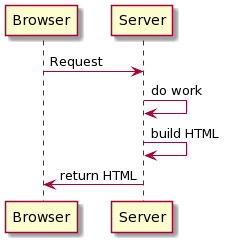
\includegraphics{browserToServer}

The browser would request a web page and the server would do some work to hand build it.  Inevitably as more browsers came online, and more browser versions came online, more and more work had to be performed by the server developers to tailor to issues with content rendering in various browsers. Mostly fighting Internet Explorer.  Additionally, as web content became more and more complex, so did the code to build the customized reply for shopping carts, bank statements, flight status, etc.

Eventually, server developers started adopting frameworks such as ASP.NET (C++) or JSPs (Java) which isolated built parameters with HTML response content:

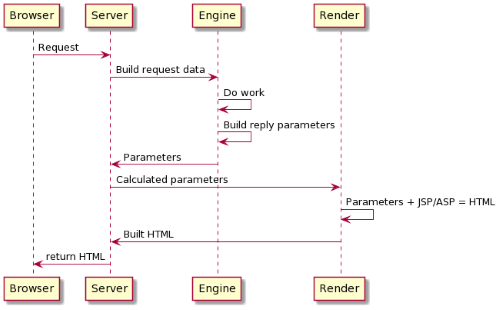
\includegraphics{jsps}

Anyone with experience building JSPs and ASPs knows it actually works a little different, such as JSP and Java getting compiled into a single .class file which is treated as both the renderer and the engine, but for the history lesson, the process is more important than the actual artifact.

With this update, we began the process of isolating calculated output from the rendered view.  It was our first step into MVC (Model-View-Controller), but we still faced issues of page content becoming more and more complex being tailored to more and more browsers.  More than that, we had a nasty problem of scale.  In this situation, the server receiving the request would have to do the work, build the page, and fire the reply in a timely manner.  To scale, we needed to enable server-to-server communication.

Our first dive into server-to-server involved custom socket buffer definitions, which then migrated into Simple Object Access Protocol, aka SOAP.

\begin{sidebar}
\begin{center}
\textbf{XML, SOAP, and JSON}
\end{center}
We're going to hit on a bit of history with XML, SOAP, and JSON so it is worth having a short example of each as a TODO list.

Sample XML reply that could be considered "browser friendly":

\begin{code}
\vspace{-\baselineskip}
\begin{lstlisting}[belowskip=-\baselineskip]
<?xml version="1.0" encoding="UTF-8"?>
<todo>
  <item>Laundry</item>
  <item>Trash</item>
  <item>Dishes</item>
</todo>

\end{lstlisting}
\end{code}

With a potential SOAP equivalent:

\begin{code}
\vspace{-\baselineskip}
\begin{lstlisting}[belowskip=-\baselineskip]
<?xml version = "1.0" encoding="UTF-8"?>
<SOAP-ENV:Envelope
   xmlns:SOAP-ENV = "http://www.w3.org/2001/12/soap-envelope"
   SOAP-ENV:encodingStyle = "http://www.w3.org/2001/12/soap-encoding">

   <SOAP-ENV:Body xmlns:m = "https://www.example.com/todos">
      <m:Todo>
         <m:Item>Laundry</m:Item>
         <m:Item>Trash</m:Item>
         <m:Item>Dishes</m:Item>
      </m:Todo>
   </SOAP-ENV:Body>
</SOAP-ENV:Envelope>

\end{lstlisting}
\end{code}

Finally, our less-verbose, browser and user-friendly JSON equivalent:

\begin{code}
\vspace{-\baselineskip}
\begin{lstlisting}[belowskip=-\baselineskip]
{"todo": ["Laundry", "Trash", "Dishes"]}
\end{lstlisting}
\end{code}

\end{sidebar}

SOAP has a rather lengthy and sordid history, which is not the focus of this book, but it is worth touching upon.  SOAP was a rather loose concept of standardizing XML, conveying context such as username and passwords, the request, and the action being performed.  All of it was XML and different architects would inevitably have very different approaches.  Context information such as session, user, password, and more could be found as HTTP Headers, within the SOAP Envelope, or even within the SOAP Body.  SOAP was verbose, machine-friendly, JavaScript unfriendly, not very developer-friendly, and fragmented.  There are certainly more issues with SOAP, but you get the point.

\begin{minipage}{\linewidth}
So, with SOAP, we migrated an XML API architecture approaching something along the lines of

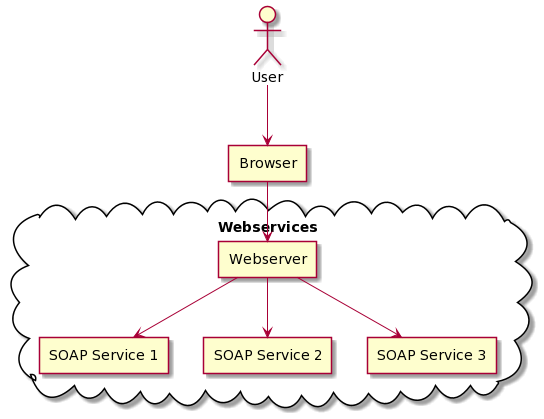
\includegraphics{soap1}

\end{minipage}

This is still before mobile phones are a thing.  The web continues to grow and users are loading up Netscape, Internet Explorer, Opera, FireFox, and others.  Content started to not only require different HTML responses but different release cycles outside of the SOAP service development cycle.  Offering up media such as CSS and image changes took an isolated release process from many of the SOAP services.  Enter Asynchronous JavaScript and XML, better known as AJAX.  AJAX + SOAP really was too much to handle, as you started to see ugly JavaScript needing to be written to handle the SOAP payloads.  More often, you'd have custom XML services talking to custom SOAP and databases.

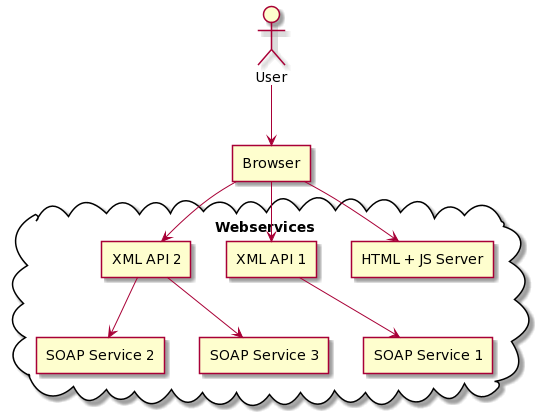
\includegraphics{soap2}

The problem compounds as the page complexity grows and now you have browser-friendly XML APIs and server SOAP APIs.  Inevitably the clients on both browsers and servers, for browser-to-server and server-to-server communication needs to become more consistent and more consumer friendly.  Concurrently to all of this nasty fragmentation, browser engineers start forcing the issue with JavaScript Object Notation (JSON).

In quick succession, smart (and staffed) companies pull this stunt:

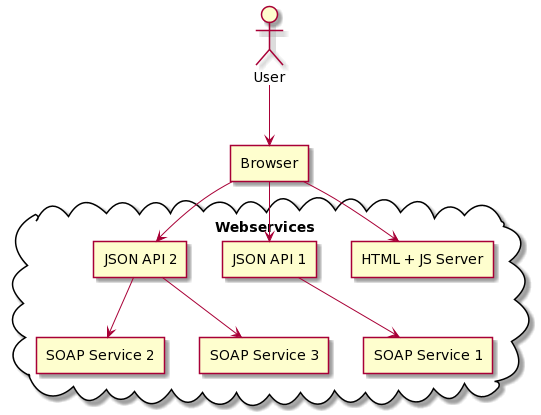
\includegraphics{js1}

followed by

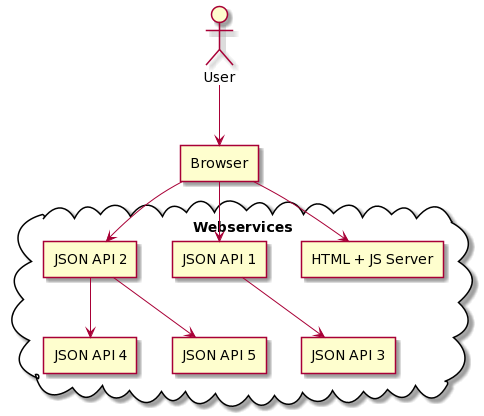
\includegraphics{js2}

Next step was just to standardize the JSON APIs, getting to that convention-over-configuration that offers enough consistency to feel common but malleable enough to answer business requirements without feeling like hammering a square peg into a round hole.  REST is the chosen victor in our arena.

Ultimately, it rapidly progresses into something luxurious that supports mobile clients, browser clients, internal server-clients, customer servers, API gateway proxies, geo-distributed content delivery networks (CDNs), with RESTful APIs providing the majority of server-state to all interested consumers.

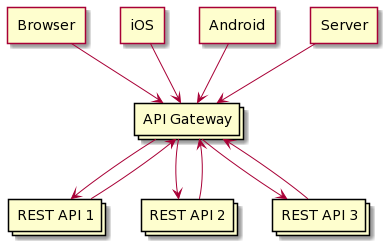
\includegraphics{modern}

\begin{sidebar}
\begin{center}
\textbf{Hidden Services}
\end{center}

Do note, this diagram is completely missing big ticket items like scalable block storage, databases, eventing systems, messaging systems, and more.  The point being made is that client-to-server and server-to-server communication channels moved from fragmented APIs and standards to consistent channels of REST communication.

\end{sidebar}

\section{Case Study: Library}

Throughout the remainder of this text, we will leverage a case study to design an API with the Open API 3.0 specification.  Our project is to design an API for administrators and consumers of a library.  User stories will include book check-in, book check-out, lost books, sold books, and book availability.  The list of user stories is offered here to allow you to have foresight into where we will take this project, but it is not required you go through them now.  Certainly, don't get ahead of yourself and begin planning out the API just yet.

\begin{itemize}
  \item I as a Borrower need to check on a book's availability so that I may know if the book I wish to checkout is available.
  \item I as a Borrower need to search for a book by title so that I may know if the book I wish to checkout is available.
  \item I as an Admin need to reserve a copy of a book for a patron so that they may know it is available when they arrive.
  \item I as an Admin need to create a book so that I may prepare incoming purchased books for borrowing.
  \item I as an Admin need to mark a book as sold so that I may remove sold book copies.
  \item I as an Admin need to create a borrower account so that I may enable new borrowers.
  \item I as an Automated System need to find past-due books so that I may notify borrowers of fines and fees.
\end{itemize}

Obviously, this list is entirely incomplete of what services would be required for a full library service offering.  You'd need user search features, account administration features, administrator administration features, payment services, and more.

Our identified actors include:

\begin{itemize}
  \item Admin: Your friendly librarian.
  \item Borrower: Anyone interested in checking out books.
  \item Automated System: A running application or batch process; just code that does regular work be it scheduled or on-demand.
\end{itemize}

\chapter{Basics of Modeling REST}

As we dive into modeling the API for our first user stories, we'll be using Open API 3.  You can find the latest resources for Open API 3 at \url{https://github.com/OAI/OpenAPI-Specification}.  Take note that there is both a community and a business behind this modeling specification, \url{https://smartbear.com/}, and they are deserving of support.  The fastest way to begin modeling your API is by using their resources at \url{https://editor.swagger.io/}.

\begin{sidebar}
\begin{center}
\textbf{Open API 3}
\end{center}

We will leverage Open API 3 specification to model our REST API, but this is not a book diving into the full specification of it.  You can read the full specification in an hour and it is worth doing so after you've ready this book.  Our goal here is to present a model of REST endpoints without selecting a programming language to implement it in.  There are a few leaders in the modeling options including RAML, Open API 3, Swagger 2, and API Blueprint.  Visit \url{https://github.com/OAI/OpenAPI-Specification} for the full specification.

\end{sidebar}

When modeling a RESTful object state, pay careful consideration to the object state being akin to naming and describing a noun.  You should not have a component definition of GetSearchResult, it would just be SearchResult.

\begin{sidebar}
\begin{center}
\textbf{Object State, Component, or Resource?}
\end{center}

Our modeling markdown choice of Open API 3.0 uses the label "component", REST labels it "state", and URL is an acronym for Uniform \underline{Resource} Locator.  \textit{We will use component, resource, and object state interchangeably when discussing modeling the RESTful object's properties.}

\end{sidebar}

\section{Modeling REST Object State}

User Stories we will start with for resource modeling:

\begin{itemize}
  \item I as a Borrower need to check on a book's availability so that I may know if the book I wish to checkout is available.
  \item I as a Borrower need to search for a book by title so that I may know if the book I wish to checkout is available.
  \item I as an Admin need to reserve a copy of a book for a patron so that they may know it is available when they arrive.
\end{itemize}

Based on these three user stories, we can go through and determine the resources we need to model.  We know we have a Book, or really a book's metadata.  We also know we have to model the physical copy of a text, such as a uniquely scannable barcode for a library to check-in and check-out.  We can then speak to our product owner regarding restrictions for the availability search.  Must the user be authenticated, or can an anonymous user inspect the availability for a certain title?  In this case, we're going to allow any unauthenticated user to research a book's availability.

Let's start with some assumptions based on fictitious conversations with our product owner.  For our book, we know that we want to include title, authors, copyright date, and International Standard Book Number (ISBN-13).

\begin{minipage}{\linewidth}
We can start by modeling the applicable resources using Open API 3.0 YML.  This component YML can be placed within the editor at \url{https://editor.swagger.io} and you can review how the resulting object will look.
\begin{code}
\begin{lstlisting}[belowskip=-\baselineskip]
components:
  schemas:
    Book:
      type: object
      properties:
        isbn:
          type: string
          description: International Standard Book Number
          example: 978-1119096726
        title:
          type: string
          description: Book title
          example: Applied Cryptography
        authors:
          type: array
          items:
            type: string
          example: ["Bruce Schneier"]
        copyrightDate:
          type: integer
          example: 2015
\end{lstlisting}
\end{code}
\end{minipage}

\begin{sidebar}
\begin{center}
\textbf{JSON CamelCase, Dashes, or Underscore?}
\end{center}

It is left up to the API designer to choose between camelCase, kebab-case (dashes), or underscores for separators.  That said, Google's JSON Style Guide at \url{https://google.github.io/styleguide/jsoncstyleguide.xml?showone=Property_Name_Format#Property_Name_Format} standardizes on camelCase.  We will follow camelCase for our JSON definitions.

\end{sidebar}

\begin{sidebar}
\begin{center}
\textbf{Yet Another Markup Language}
\end{center}

YAML, pronounced yam-el, is short for either "Yet Another Markup Language" or the recursive "YAML Ain't Markup Language" depending on who you ask.  It is becoming more and more common for specification and configuration files.  Golang, Python, Java, and others have parsers for it.  It is the most common configuration format for Spring Boot, now emitted by the Spring Boot initializers by default.  At its core it has the look and feel of Python because space matters, but it is a very clean, readable, and concise markup for configuration and now Open API 3.0 specification.

\end{sidebar}

So, with our book resource defined, we know we need to add a list of available copies.  So, why can't we just put a list of copies on the Book resource itself?  The argument can even be made in the is-a vs has-a relationship OOP model that a copy of a book is-a book, so from a polymorphic language a book copy could just inherit from Book.  You would be correct.  However, when we're modeling our REST endpoint URLs, searching for books by title vs retrieving available copies by ISBN will have different URL paths.  It would be completely acceptable to start modeling resources, then get to the endpoints, and come to the conclusion that when modeling your endpoints you want to split up the object instead of treating it as an inherited object.  An Object-Oriented Programming (OOP) purist would even struggle with the Book labeling, and show that it should really be something along the lines of BookMeta, or BookDescriptors.

\begin{minipage}{\linewidth}
\begin{code}
\begin{lstlisting}[belowskip=-\baselineskip]
components:
  schemas:
    BookCopy:
      type: object
      properties:
        isbn:
          type: string
          description: International Standard Book Number
          example: 978-1119096726
        barcode:
          type: string
          description: Copy identifier used for scanning and unique text copy result.
\end{lstlisting}
\end{code}
\end{minipage}

By including the ISBN in our BookCopy, we're violating data duplication tenets of OOP.  Again the question comes up, does a BookCopy have a Book?  Technically, we're not in OOP here.  When we're modeling object state for REST, we want lean results, driven by consumer needs.  On the one hand, OOP would decry this approach.  In our case, we want to be mindful of the fact that the Book object may grow and grow, impacting network costs when returning say an array of BookCopy results when providing an endpoint for all of the available copies assigned to a library.  Imagine the Library of Congress, which could have 50 copies of \textit{Catcher in the Rye}.  If I was to request all BookCopies for \textit{Catcher in the Rye}, I would not want the full Book object embedded within every element of the array.  The reality is, this is a bit of a balancing act.  You could also strip away the referential ISBN between BookCopy and Book, but then you would have no means to scan a book's barcode, look up the copy by barcode, and relate it to a Book.

That feeling of "that's not right", is because we're breaking typical OOP, and there are no hardened rules here.  Networking costs, balancing referential data between objects, staying focused on client user stories, it is a bit of a complex burden.  For such a simple, ancient problem of modeling and architecting a library's set of RESTful endpoints, there's a lot to consider and a lot to model.

All of that said, we're still at an awkward place in terms of defining number of available copies.  Would we include available count on the Book?  Well that's not the right place because we've chosent to split up Book and BookCopy.  Would we include available count on a BookCopy?  Well no, we expect a book copy to be singular.  What we're uncovering is that we have a read-only object to define, a resulting resource from a search.  You will commonly find that search results require a defined component which feels out of place because it won't map into your back-end system's object storage.  This is where the back-end focused architects may struggle and where consumer-driven-contracts becomes key.  We care about our consumers' needs first.  That said, our result needs to be a search result.

\begin{minipage}{\linewidth}
\begin{code}
\begin{lstlisting}[belowskip=-\baselineskip]
components:
  schemas:
    BookAvailability:
      type: object
      properties:
        isbn:
          type: string
          description: International Standard Book Number
          example: 978-1119096726
        available:
          type: integer
          minimum: 0
          description: Available copies for checkout or reservation, ranging from 0 to N
        checkedOut:
          type: integer
          minimum: 0
          description: Total copies checked out
\end{lstlisting}
\end{code}
\end{minipage}

Looking at this BookAvailability definition for a search result, we would have a debate over if the result should include ISBN.  Let's suppose that we are planning to provide an endpoint to find available copies by ISBN, why would we echo the ISBN back?  If there's a reason, why not just echo the entire Book component back and include the title, the author, etc.

Again, this is where a choice of style comes into play, and engineers will disagree.  My opinion is that when our browser-based clients are constructing asynchronous JavaScript processing results in promise blocks, debugging will be much easier for them if there is a reference between search result and search text.  Developer tools showcasing the network request/response data will also be easier to trace when including relational data.  Should the relational data be the full Book component?  Perhaps, but you can also make the case that the Book will likely grow and grow over time and feature requests, say maybe include pages, publisher information, secondary publishing details, etc.

There are merits to include the ISBN, not include the ISBN, and provide a full embedded result of the Book that was used for searching available copies.  All three are right, and all three have reasons to be wrong, and that tells us that some of our decisions here are going to be Artistic and not Scientific.

If these modeling decisions were left to a committee of architects, I'd anticipate quite a bit of argument here.  The joys of having too many cooks in the kitchen.

\emph{Object Modeling Summary:}

\begin{itemize}
  \item Use Consumer-Driven Contracts over Object Oriented Programming to design your objects.  We're not in OOP anymore.
  \item Designing RESTful object state is as much art as science.
  \item Object state should be labeled as a resulting noun (person, place, or thing) and not be prefixed by a verb for the interaction.  Use Book instead of GetBook.
\end{itemize}

\section{HTTP Methods and REST}

When speaking to or as a system architect, HTTP Methods are known as REST Verbs.  It is the action you are taking against the resource.  You're posting it, getting it, putting it, or deleting it, so the terminology is appropriate.  HTTP Method and REST Verbs are interchangeably used in REST API architecture conversations.

The most common RESTful verbs for mapping out create-read-update-delete (CRUD) operations are GET, PUT, POST, and DELETE.  There is a lesser known PATCH operation used as well, which serves as a sparse data update.  Finally, you will encounter OPTIONS when using REST services from a browser, particularly when going across domains, say from www.example.com hitting an API offered using a subdomain such as rest-api.example.com.

To provide a quick preview, HTTP GET is object retrieval or collection search, and shouldn't incur any side effects.  It is imperative, from a security perspective even, that HTTP GET methods inflict no change.  Why?  The fastest answer to give would be that some services still leverage long-lived session cookies for user identity.  Imagine I am a customer at a bank, and they have my authenticated session stored as a cookie in my browser, and I happen upon an emailed link which works along the lines of \textit{/transfer/to?account=hackers\&amount=500.00} which says "click to see video here" as the presented text in the email.  Bad day.  Just don't incur changes to object state as a GET.

HTTP POST is meant for resource creation.  HTTP PUT is for resource update \textit{or resource creation}.  HTTP DELETE is for deletions or cancellation.  Finally, HTTP PATCH should be used for a sparsely filled updates against large resources, or content that is easier for the client to update portions of the resource instead of the whole resource.  Expect a much more thorough explanation in the coming chapters.

\begin{minipage}{\linewidth}
\begin{sidebar}
\begin{center}
\textbf{Security First}
\end{center}

The security aspects of designing a RESTful API are presented within this book after presenting the foundational concepts.  This is not the correct approach to take when designing an API.  Security must be a first class citizen when preparing RESTful services.  Whether secured via an API gateway enforcing access controls or building a zero-trust network of microservices, know your security approach before you start implementing.  Retrofitting security into insecure APIs is a mistake and one that could cost your company dearly.  Your clients will need to know your identity provider, you will need to know how to validate the principal, you will need to know how to determine level of authorization, and you will need to have a plan for non-prod test accounts and test credential automation for integration testing.

\end{sidebar}
\end{minipage}

\emph{Method Summary:}

\begin{itemize}
  \item HTTP Methods GET, PUT, POST, DELETE, and PATCH are also known as REST verbs.
  \item HTTP GET methods are read-only must incur no side effects to the object state.
  \item HTTP POST is create.
  \item HTTP PUT is update or create.
  \item HTTP DELETE is deletion or cancellation.
  \item HTTP PATCH is sparse update.
\end{itemize}

\section{Modeling Endpoints}

When designing your REST endpoint, start by identifying the nouns which we can describe state for.  In our case study, we have books and book copies.  In a much more complete application plan, we'd also have users, libraries, publishers, and potentially more.  Start by determining the object states your consumers are going to need to retrieve, and then model that as a collection.  For example, \textit{/books} and \textit{/copies}.  When describing a collection of resources such as books or copies, use the plural in the URI and treat the identifier as a path component.  For example, \textit{/books/book-id} and \textit{/copies/copy-barcode}.

One thing a good system architect will always be ready for is change.  We plan for it because we know it will inevitably happen, either from design mistakes, technology updates, changes in feature requirements, new feature additions, etc.  Designing REST can set the level of preparedness for the inevitability of change.  We will version our endpoints, assuming that contract breaking changes will happen over the coming releases.  A hot topic will be do we place the version in the endpoint URL, or do we make use of HTTP Headers, or do we make use of subdomains.

Three options commonly available:

\begin{itemize}
  \item http://www.example.com/v2/books/book-id
  \item http://v2.example.com/books/book-id
  \item http://www.example.com/books/book-id + HTTP Header such as X-Version: 2.0
\end{itemize}

My recommendation will be that you place the version in the URL, so \textit{/v2/books/book-id}.  The benefits include:
\begin{itemize}
  \item Our site access logs will include both the version of the API and the HTTP status code, so we can quickly tell if we're getting HTTP status errors from an old version or a newer one, particularly during updates to our API suite.
  \item We can document multiple versions within the same Open API 3.0 contract document.
  \item An API Gateway can easily route traffic based on URL.
  \item Common REST frameworks, such as Spring Boot, can isolate controllers by version of the API.  This will allow one application to process both contract versions.
\end{itemize}

Our choice of placing the version into the URL is Art over Science, as all three flavors of versioning are viable.  The most important takeaway is that you plan for change and have versioning prepared in your API contract at the very first iteration.  I warn that there are architects who will disagree with the recommendation to include version in the URL and expect the version to be an HTTP header because the version is contextual; they're right.  There are others that will want the version to be placed in the domain, so they can manage routing the request by domain; they too are right.

\section{Consumer Driven Contracts}

A core API design tenet to touch upon before we start designing our API is Consumer Driven Contracts, which we will use throughout our design process.  Presenting theory for the pattern for Consumer Driven Contract is quite simple:  \textit{the consumer's needs drive the contract of the resulting API.}

The idea of Consumer Driven Contracts is not new to REST API engineers.  Many SOAP and other TCP services are built with the consumer in mind, but it is worth revisiting for architects planning out RESTful APIs.  At its core, the concept of Consumer Driven Contracts places the burden on the back-end engineers to write the service once, so that the N number of client integrators don't have to rewrite the business logic to accomplish the same task.  The ideal thin client is facilitated by a clean API answering its requirements sufficiently and cleanly.

While the architect for APIs tends to be experienced back-end systems engineers, there is quite a bit of merit to assigning the front-end engineers as the designers. Consumer-Driven Contracts places the burden on the back-end teams to develop systems which hide the complexity through a consumer friendly API. We will hide all of the legacy, all of the technical debt, and all of the poor technology choices behind a clean API meant to enable clients to quickly integrate to.

Our goal for clients is fast adoption so that we can build native and browser apps for Android, iOS, desktop, and command-line consumers.  In addition, thought is given to scenarios where your consumers may be other microservice apps.

When designing an API, it is imperative you have a notion of your consumers, be them microservices, native clients, or terminal system admins.  More importantly, even if you're the developer working on the back-end providing the API offering, you must know the user stories and use cases driving the need for your implementation. Take for example the following user story for a library:

\textit{I as a library administrator need to determine the availability of a book by ISBN so that I may answer availability questions regarding a title.}

This user story could lead to a very different API offering than:

\textit{I as a system need to obtain the list of book copies by ISBN so that I may determine if too many books have been purchased and should be offered for sale.}

The librarian needs to know what's available right now, but the system may need how many are checked out and how many are owned by the library in total.  You can answer both needs with the same REST endpoint, but notice how the system story expands the scope of the resulting API to include copy counts.  Proper planning given into the final API may result in reduced work performed by the system teams to cover the breadth of the user stories.

The argument can be made that this approach smells like a waterfall planning model verses feature planning for an Agile sprint, and you'd be correct.  That said, an architect with a few discussions with a product owner can plan out a strong API in a single sprint, without having to scope the entire project out in a waterfall model.  That doesn't mean the API won't change, and that doesn't mean the API will be perfect, but the planning can pay off in big ways.

\section{Consistency is Key}

Chances are, when planning out your API's context that most of what you're doing isn't unique.  It has been done before and chances are it has been standardized and documented.  Leverage web searches to find common header HTTP header labels and HTTP status codes.

If you're looking for an appropriate status code for your client's failure, say from providing an expired authentication, that's going to be a 401 and you're quickly led to that conclusion with a quick search.  You can find a quick run-down of common status codes at \url{https://developer.mozilla.org/en-US/docs/Web/HTTP/Status}.

For tracing and correlation of requests and client session activity, it has again been done before.  See \url{https://en.wikipedia.org/wiki/List_of_HTTP_header_fields} which will lead you to \textit{X-Request-ID} and \textit{X-Correlation-ID}.

The point is that if what you're designing is primarily contextual or technical, not related to your API's custom object state, try to stick to common headers and status codes.  Your consumers will thank you for it.


\chapter{First Models}

\section{REST GET}

We will design our first REST GET endpoint by starting with our user story.

\textit{I as a Borrower need check on a book's availability so that I may know if the book I wish to checkout is available.}

From this story, we can tell we want an endpoint to retrieve our BookAvailability resource.  Reaching out to our product owner, we query whether or not we would assume this shows up as part of a book search by title, or if we can assume they already have the unique ISBN.  For our purpose, we will assume a search has been a performed, the user selected from a list of matching titles, and now the client has the ISBN.  What we're looking to design here is the URL for book copy availability by ISBN.

When modeling URLs for REST, there are many considerations to make.  First, is there one resource or multiple resources of the same type?  If the resource is plural, the URL should include a plural, such as /v1/books, or /v1/copies.  Second, is the operation uniquely identified by an identifier, meaning a result of one, or is it retrieval of the list of resources?  If a filtered list with potentially multiple non-unique results, use query parameters such as \url{/v1/books?title=REST}.  If we are looking to identify a unique book, we could model \textit{/v1/books/\{isbn\}} as our URL.

Probably the trickiest portion of modeling a REST API's URLs is relative pathing for relational resources.  Take for example our BookCopy resource being a copy of a Book.  We could potentially model our URLs as \textit{/v1/books/\{isbn\}} and \textit{/v1/copies/\{isbn\}}.  We can also consider the relational aspect of a copy to a book and make copies a sub resource of books, such as \textit{/v1/books/\{isbn\}/copies}.  A guideline here is, \textit{choose the URL which is easier for the consumer to understand}.  If you took the \textit{/v1/copies/\{isbn\}} by itself, it isn't very expressive regarding a copy of what.  However, \textit{/v1/books/\{isbn\}/copies} is much more expressive indicating we're looking at copies of a book.

\begin{minipage}{\linewidth}
Choosing the more expressive endpoint, we can now model our happy-path book availability URL:

\begin{code}
\begin{lstlisting}[belowskip=-\baselineskip]
paths:
  /v1/books/{isbn}/copies:
    get:
      summary: Retrieve available copies of a given Book
      operationId: retrieveAvailability
      parameters:
      - name: isbn
        in: path
        description: ISBN-13 book identifier
        required: true
        schema:
          type: string
      responses:
        200:
          description: ISBN found, server able to identify available copies of book identified by ISBN.
          content:
            application/json:
              schema:
                $ref: '#/components/schemas/BookAvailability'
\end{lstlisting}
\end{code}
\end{minipage}

Now we've modeled our object state as well as URL for checking on availability.  Let's move on to our search story.

\section{Search Results}

\textit{I as a Borrower need to search for a book by title so that I may know if the book I wish to checkout is available.}

Given we've already defined an endpoint of \textit{/v1/books/\{isbn\}/copies}, we can see we're not looking to search for copies, we're looking to search on books.  Our endpoint for REST modeling here would be attached to \textit{/v1/books}.  We're looking to model a search capability for our Borrower actor, and we know they don't know the ISBN off of the top of their head.  When you can't uniquely identify the resource by ID and your case requires filtering or searching, use query parameters.   In this case, we will model the endpoint with a title query parameter.

\begin{minipage}{\linewidth}

\begin{code}
\begin{lstlisting}[belowskip=-\baselineskip]
/v1/books:
  get:
    summary: Search for books
    operationId: searchBooks
    parameters:
    - name: title
      in: query
      description: Title match for book search
      required: true
      schema:
        type: string
    responses:
      200:
        description: Matching titles found
        content:
          application/json:
            schema:
              type: array
              items:
                $ref: '#/components/schemas/Book'
\end{lstlisting}
\end{code}
\end{minipage}

Reviewing our resource, we can question how many matches could we afford before it becomes a problem.  What happens if our user searches for "The"?  Coordinating with product owner, our library search feature is problematic because we can't answer with the entire library in a single HTTP response, and the UI direction is to allow for drop-down matching when additional letters are typed.  Let's generate a paged result component for the search result.

\begin{minipage}{\linewidth}

\begin{code}
\begin{lstlisting}[belowskip=-\baselineskip]
BookSearchResultPage:
  type: object
  properties:
    totalMaches:
      type: integer
      description: Total number of matched books
    limit:
      type: integer
      description: Maximum number of books returned in a paged result
    offset:
      type: integer
      description: Matching Book offset for pagination
    books:
      type: array
      items:
        $ref: '#/components/schemas/Book'
      description: Matching books
\end{lstlisting}
\end{code}
\end{minipage}

And to enable our consumers to make use of the paging result, we'll update our search endpoint:

\begin{minipage}{\linewidth}
\begin{code}
\begin{lstlisting}[belowskip=-\baselineskip]
/v1/books:
  get:
    summary: Search for books
    operationId: retrieveBooks
    parameters:
    - name: title
      in: query
      description: Title match for book search
      required: true
      schema:
        type: string
    - name: offset
      in: query
      description: Match offset for retrieving next page of matching titles
      required: false
      schema:
        type: integer
    responses:
      200:
        description: Matching titles found
        content:
          application/json:
            schema:
              $ref: '#/components/schemas/BookSearchResultPage'
\end{lstlisting}
\end{code}
\end{minipage}

\emph{HTTP GET Summary:}

\begin{itemize}
  \item HTTP GET is for read only services and must not trigger object state change (side effects)
  \item Model your resource URLs such that they are relative in the path when related, such as our \textit{/v1/books/\{isbn\}/copies}
  \item When uniquely identifying a resource, the ID belongs on the URL path.  When filtering or searching for a matching set of resources, use query parameters.
\end{itemize}

\section{REST POST}
\section{REST PUT}
\section{Idempotent PUT vs POST}
\section{REST PATCH}
\section{REST DELETE}


%%% WIP Outline
\chapter{Status Codes}
\section{1xx-5xx}
\section{Success!}
\section{Bad Client!}
\section{Bad Server!}

\chapter{Headers and Context}
\section{Client Information}
What client?  Who's the bad client implementation?
Big sidebar on tracing client for notifying who needs to update.  MTR reference story
\section{Tracing and Correlating}
X-Request-ID, X-Correlation-ID
\section{Authentication}

\chapter{Securing Your Traffic}
\section{TLS and MitM}
\section{TLS Issuance Services}
letsencrypt.org
\section{Self Signed Certificates}
\section{SSL is Dead, Long Live SSL}
TLS vs SSL.  POODL, SSL v3 is dead topic.

\chapter{Securing Identity}
\section{Authentication vs Authorization}
\section{Non-Repudiation}
\section{Basic Auth}
\section{Bearer Auth}
What is a JWT?
\section{Mutual TLS}
\section{OIDC, OAuth}

\chapter{Browser Awareness}
\section{Cookies vs Headers}
\section{CORS Preflight}
Why can't I hit my API from swagger?

\section{Options Denied!}
\section{HTML 5 Storage}

\chapter{Secure Architecture with CI/CD}
\section{Continuous Integration, Continuous Delivery}
\section{Backdoors for Testing}
\section{Zero Trust vs Segregated Environment}
\section{Future of REST with HTTP 2.0}
Modeling Websockets

\chapter{REST Deployment Architecture}
\section{Architecture}
\section{API Gateways}
Apigee, API Gateway, Tyk.io
\section{CQRS}
\section{Eventing and Websockets}
No modeling leader here.

\chapter{Alternative Modeling}
\section{Swagger 2}
\section{RAML}
\section{WRML}
\section{API Blueprint}

\chapter{Appendix}
\section{Monolithic Decomposition}
\section{Microservices and Containers}
\section{Function-as-a-Service}
\section{HATEOS}
\section{Library Modeled in Open API 3.0}

%% TODO:
%% Build skip fail if file unlinked
%% Hammer in a why can't I hit my endpoint?

\begin{thebibliography}{9}

\bibitem{fielding}
Roy Thomas Fielding
\textit{Architectural Styles}
University of California, Irvine, 2000.

\bibitem{Jennings}
Richi Jennings
\textit{Scraped Parler data is truly revealing}
\url{https://techbeacon.com/security/scraped-parler-data-reveals-countless-capitol-perps}, 2021.

\end{thebibliography}


\end{document}


%%%% NOTES
%\begin{sidebar}
%\begin{center}
%\textbf{Disclaimer}
%\end{center}
%This is some command
%These commands are interesting
%\end{sidebar}

%\begin{code}
%This is some code
%\end{code}
